%! Author = tstreule

\section{SPECT \textnormal{-- Single Photon Emission CT}}

$\textrm{SNR} \propto \sqrt{\textrm{total \#detected gamma-rays}}$
%%%%%%%%%%%%%%%%%%%%%%%%%%%%%%%%%%%%%%%%%%%%%%%%%%%%%%
\subsection{Radioactivity in the body}
%
\highlight{$Q = -\frac{dN}{dt} = \lambda \cdot N \implies N(t) = N_0 \eu^{-\lambda t}$}\\
$[Q] = \unit{Curie} = \unit{Ci} = 3.7 \cdot 10^{10} \unit{Bq}$
\quad where \quad $1\unit{Bq} = 1\unitfrac{disintegration}{s}$

\textbf{Physical} $t\ped{1/2} = \frac{\ln 2}{\lambda}$, \quad \textbf{biological} $t\ped{1/2 bio} = \frac{\ln 2}{\lambda\ped{bio}}$

$N(t) = N_0 \eu^{-(\lambda + \lambda\ped{bio}) t} = N_0\eu^{-\lambda\ped{1/2 eff}t}$
\quad where \quad $t\ped{1/2 eff} = \frac{t\ped{1/2} \cdot t\ped{1/2 bio}}{t\ped{1/2} + t\ped{1/2 bio}}$

\textbf{$\gamma$ photons: Absorption} or \textbf{Scattering}: Change of direction by $\theta$. \highlight{$E_{\gamma}' = \frac{m_e \cdot c^2}{m_e c^2 / E_\gamma + 1 - \cos \theta}$}
%%%%%%%%%%%%%%%%%%%%%%%%%%%%%%%%%%%%%%%%%%%%%%%%%%%%%%
\subsection{Interaction of $\gamma$ photons with matter}
%
\textbf{Absorption} leads to ejection of orbital electron\\
\textbf{Scattering}: Change of direction by $\theta$. \highlight{$\displaystyle E_{\gamma}' = \frac{m_e \cdot c^2}{m_e c^2 / E_\gamma + 1 - \cos \theta}$}
%%%%%%%%%%%%%%%%%%%%%%%%%%%%%%%%%%%%%%%%%%%%%%%%%%%%%%
\subsection{Anger Camera}
\textbf{Collimation} necessary $\implies$ losses of 99.9\%

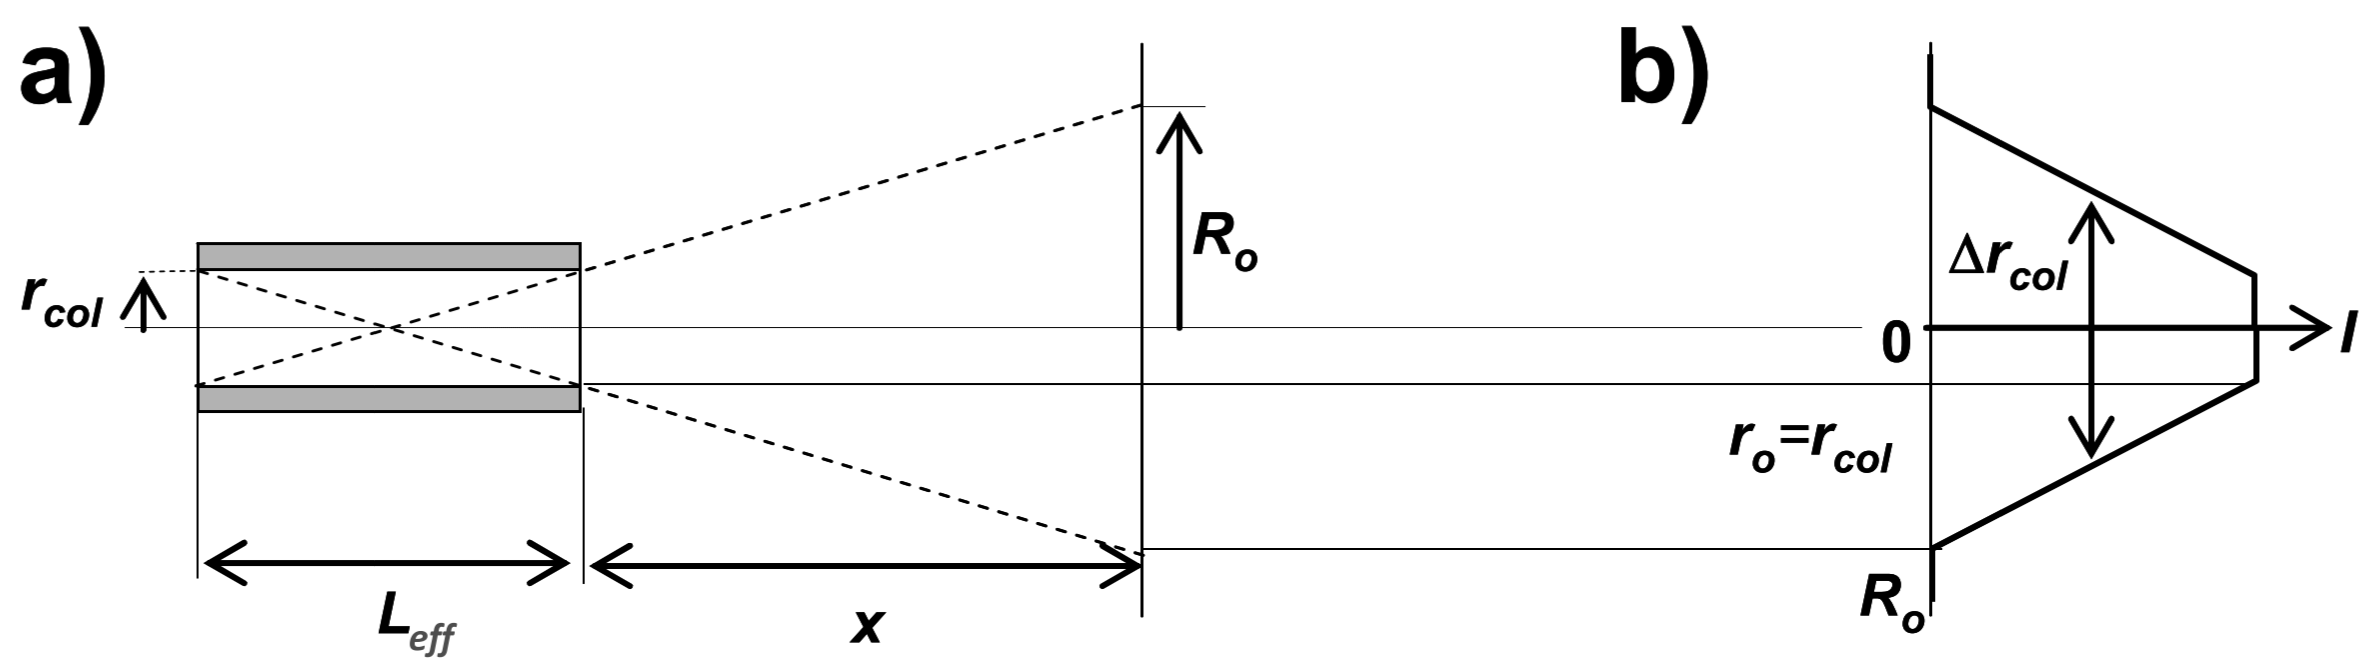
\includegraphics[width = \linewidth]{SPECT_NuclearCollimator}
Bad isolation of \textbf{septa} (lamellae) $\implies L\ped{eff} = L - \frac{2}{\mu\ped{septa}}$\\
%
\highlight{$\displaystyle R_0(x) = \frac{2 r_{col}}{L_{\text{eff}}}(x + \frac{L_{\text{eff}}}{2})$} \; \highlight{$\displaystyle \textrm{FWHM} = \Delta r_{col}(x) = \frac{2 r_{col}}{L_{\text{eff}}}(x + L_{\text{eff}})$}\\

\textbf{Signal Path}: $\gamma$-rays @140keV $\to$ Scintillation crystal $\to$ PMT $\to$ (Pos. network || pulse height analyzer) $\to$ digitizer
\begin{itemize}
    \item Scintillation crystal efficiency: \highlight{$\displaystyle \epsilon = 1 - \eu^{-\mu d}$}. $\mu$: attenuation coefficient of crystal, $d$: its thickness

    \item Usually many PMTs per crystal. Positioning network calculates where the event in the crystal was.

    \item $U_{PMT} \propto \gamma$ energy. Scattering $\implies$ $E\ped{scattered photons}\downarrow$. Pulse height analyzer has energy window $\Delta E$ around $E_0$.

    \item Poisson distributed $P_n(N)\vert \sigma^2 = \mu \implies \highlight{SNR = \sqrt{\mu}}$

    \item \textbf{Spatial resolution}: $R_{system}^2 = R\ped{gamma}^2 + R_{coll}^2$ \quad $R\ped{gamma}$ = uncertainty of positioning network. $R\ped{coll}$ see above.
\end{itemize}

\textbf{CT Version}: Res.: best at edge, worst in center. $\approx$ 7mm\\

For small objects: Use \textbf{pinhole} (cone-shaped, tungsten) camera: Problem: more dose needed, ``transparency'' around hole
%%%%%%%%%%%%%%%%%%%%%%%%%%%%%%%%%%%%%%%%%%%%%%%%%%%%%%
\subsection{Generation of Technetium}
No cyclotron needed, only generator: Essentially \ce{^{99}_{42}Mo} ($\unit[67]{h} \;\widehat{=}\; \unit[2.9\E{-6}]{s^{-1}}$) decays into \ce{^{99}_{43}Tc} ($\unit[6]{h} \;\widehat{=}\; \unit[3.1\E{-5}]{s^{-1}}$)

\textbf{Kinetic equations}:\\
$\deriv{~}{t}N_{Mo} = -k_{Mo}N_{Mo}$ and $\deriv{~}{t}N_{Tc} = k_{Mo}N_{Mo} - k_{Tc} N_{Tc}$\\
\highlight{$\displaystyle \implies N_{Tc}(t) = N_{Mo}(0) \frac{k_{Mo}}{k_{Tc} - k_{Mo}} (e^{-k_{Mo}t} - e^{-k_{Tc} t})$} {\scriptsize exp. decay}
